\documentclass[mathserif
,handout
]{beamer}
\usepackage{l16cn}
\usepackage{beamer-cris-style/cris_style}
\makenoidxglossaries
\loadglsentries{definitions}


\title[AIChE 2017 - Minneapolis, MN] % (optional, only for long titles)
{{\bf Control with Soft Feedback in Social Systems}}
\subtitle{\footnotesize Mathematical Principles, Empirical Evidence, and Applications}
\author[Luo, et al.] % (optional, for multiple authors)
{{\bf Yu~Luo}\inst{1} 
\and Garud~Iyengar\inst{2} \and Venkat~Venkatasubramanian\inst{1}\inst{2}
}
\institute[Columbia University] % (optional)
{
  \inst{1}%
%  {Doctoral Advisor: Prof. Venkat Venkatasubramanian}\\
%  {Co-Advisor: Prof. Garud Iyengar}\\
%  \vspace{0.25cm}
%  Complex Resilient Intelligent Systems Laboratory (CRIS lab)\\  
  Department of Chemical Engineering%\\
%  Columbia University
  \and
  \inst{2}%
  Department of Industrial Engineering and Operations Research%\\
%  Columbia University
}
\date[Oct. 29, 2017] % (optional)
{AIChE Annual Meeting \rule[-0.4ex]{0.2ex}{1.2em} 
Oct. 29, 2017 \rule[-0.4ex]{0.2ex}{1.2em} 
Minneapolis, MN}
\subject{Chemical Engineering}


\begin{document}

\frame{\titlepage}

% !TEX root =  ../beamer_template.tex

\begin{frame}{Complex Resilient Intelligent Systems (CRIS)}
	\begin{figure}[htbp]
	   \centering
	   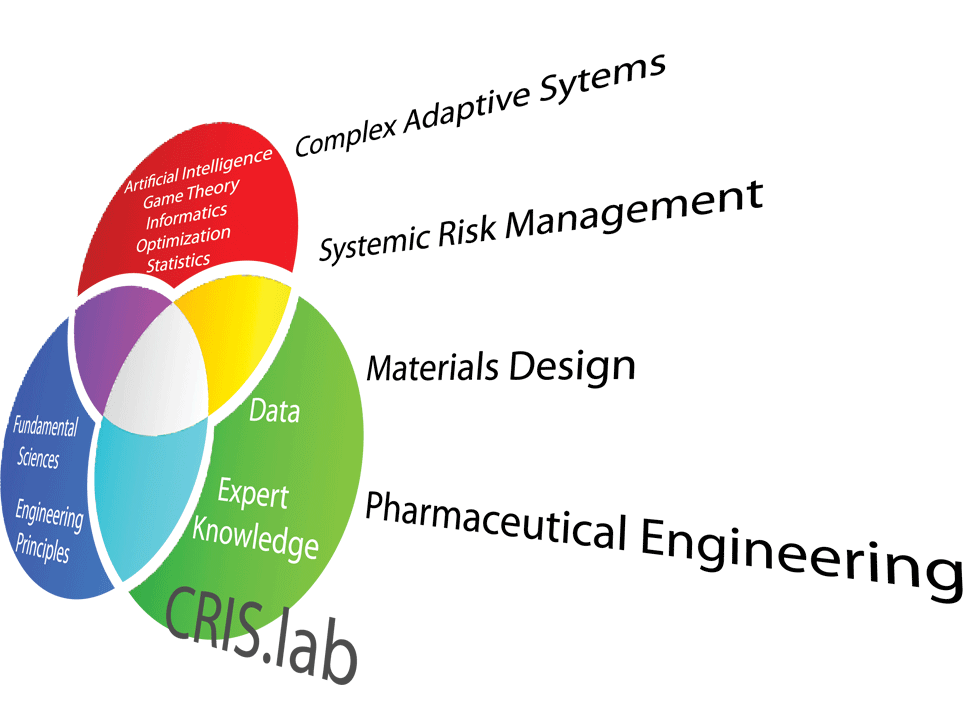
\includegraphics[width=0.75\textwidth]{fig/download/CrisResearch720.png}
	\end{figure}
\end{frame}

\begin{frame}{Overview}
	\tableofcontents
\end{frame}
\placelogofalse

\section{Introduction}
\input{beamer-sections/1_Introduction}

\section{Methods}
% !TEX root =  ../beamer_template.tex

\begin{frame}{Results and Discussion}
	\begin{itemize}
		\item Something
		\item Something
		\item Something
	\end{itemize}

\end{frame}

\section{Results and Discussion}
% !TEX root =  ../beamer_template.tex

\begin{frame}{Conclusion}
	\begin{itemize}
		\item Something
		\item Something
		\item Something
	\end{itemize}

\end{frame}

\section{Conclusion}
% !TEX root =  ../beamer_template.tex

\begin{frame}{Conclusion}
	\begin{itemize}
		\item Something
		\item Something
		\item Something
	\end{itemize}

\end{frame}

\placelogofalse
\appendix
% !TEX root =  ../beamer_template.tex

\begin{frame}{Appendix}
	\begin{itemize}
		\item Something
		\item Something
		\item Something
	\end{itemize}

\end{frame}

\end{document}
